\documentclass{report}
\usepackage{graphicx, tikz-cd, float, titlepic, booktabs} % Required for inserting images
\usepackage{amsmath, amssymb, amsthm, amsfonts, siunitx, physics, gensymb}
\AtBeginDocument{\RenewCommandCopy\qty\SI}
\usepackage[version=4]{mhchem}
\usepackage[most,many,breakable]{tcolorbox}
\usepackage{xcolor, fancyhdr, varwidth}
\usepackage[Glenn]{fncychap}
%Options: Sonny, Lenny, Glenn, Conny, Rejne, Bjarne, Bjornstrup
\usepackage{hyperref, cleveref}
\usepackage{icomma, enumitem} %comma as decimal and continue enumerate with [resume]
%%%%%%%%%%%%%%%%%%%%%%%%%%%%%%
% SELF MADE COLORS
%%%%%%%%%%%%%%%%%%%%%%%%%%%%%%
\definecolor{myg}{RGB}{56, 140, 70}
\definecolor{myb}{RGB}{45, 111, 177}
\definecolor{myr}{RGB}{199, 68, 64}
\definecolor{mytheorembg}{HTML}{F2F2F9}
\definecolor{mytheoremfr}{HTML}{00007B}
\definecolor{mylenmabg}{HTML}{FFFAF8}
\definecolor{mylenmafr}{HTML}{983b0f}
\definecolor{mypropbg}{HTML}{f2fbfc}
\definecolor{mypropfr}{HTML}{191971}
\definecolor{myexamplebg}{HTML}{F2FBF8}
\definecolor{myexamplefr}{HTML}{88D6D1}
\definecolor{myexampleti}{HTML}{2A7F7F}
\definecolor{mydefinitbg}{HTML}{E5E5FF}
\definecolor{mydefinitfr}{HTML}{3F3FA3}
\definecolor{notesgreen}{RGB}{0,162,0}
\definecolor{myp}{RGB}{197, 92, 212}
\definecolor{mygr}{HTML}{2C3338}
\definecolor{myred}{RGB}{127,0,0}
\definecolor{myyellow}{RGB}{169,121,69}
\definecolor{myexercisebg}{HTML}{F2FBF8}
\definecolor{myexercisefg}{HTML}{88D6D1}
%%%%%%%%%%%%%%%%%%%%%%%%%%%%%%%%%%%%%%%%%%%%%%%%%%%%%%%%%%%%%%%%%%%%%%
% Box environments for theorems and problems
%%%%%%%%%%%%%%%%%%%%%%%%%%%%%%%%%%%%%%%%%%%%%%%%%%%%%%%%%%%%%%%%%%%%%
\setlength{\parindent}{1cm}
%================================
% Question BOX
%================================
\makeatletter
\newtcbtheorem{question}{Opgave}{enhanced,
	breakable,
	colback=white,
	colframe=myb!80!black,
	attach boxed title to top left={yshift*=-\tcboxedtitleheight},
	fonttitle=\bfseries,
	title={#2},
	boxed title size=title,
	boxed title style={%
			sharp corners,
			rounded corners=northwest,
			colback=tcbcolframe,
			boxrule=0pt,
		},
	underlay boxed title={%
			\path[fill=tcbcolframe] (title.south west)--(title.south east)
			to[out=0, in=180] ([xshift=5mm]title.east)--
			(title.center-|frame.east)
			[rounded corners=\kvtcb@arc] |-
			(frame.north) -| cycle;
		},
	#1
}{def}
\makeatother
%================================
% DEFINITION BOX
%================================

\newtcbtheorem[]{Definition}{Definition}{enhanced,
	before skip=2mm,after skip=2mm, colback=red!5,colframe=red!80!black,boxrule=0.5mm,
	attach boxed title to top left={xshift=1cm,yshift*=1mm-\tcboxedtitleheight}, varwidth boxed title*=-3cm,
	boxed title style={frame code={
					\path[fill=tcbcolback]
					([yshift=-1mm,xshift=-1mm]frame.north west)
					arc[start angle=0,end angle=180,radius=1mm]
					([yshift=-1mm,xshift=1mm]frame.north east)
					arc[start angle=180,end angle=0,radius=1mm];
					\path[left color=tcbcolback!60!black,right color=tcbcolback!60!black,
						middle color=tcbcolback!80!black]
					([xshift=-2mm]frame.north west) -- ([xshift=2mm]frame.north east)
					[rounded corners=1mm]-- ([xshift=1mm,yshift=-1mm]frame.north east)
					-- (frame.south east) -- (frame.south west)
					-- ([xshift=-1mm,yshift=-1mm]frame.north west)
					[sharp corners]-- cycle;
				},interior engine=empty,
		},
	fonttitle=\bfseries,
	title={#2},#1}{def}
\newtcbtheorem[]{definition}{Definition}{enhanced,
	before skip=2mm,after skip=2mm, colback=red!5,colframe=red!80!black,boxrule=0.5mm,
	attach boxed title to top left={xshift=1cm,yshift*=1mm-\tcboxedtitleheight}, varwidth boxed title*=-3cm,
	boxed title style={frame code={
					\path[fill=tcbcolback]
					([yshift=-1mm,xshift=-1mm]frame.north west)
					arc[start angle=0,end angle=180,radius=1mm]
					([yshift=-1mm,xshift=1mm]frame.north east)
					arc[start angle=180,end angle=0,radius=1mm];
					\path[left color=tcbcolback!60!black,right color=tcbcolback!60!black,
						middle color=tcbcolback!80!black]
					([xshift=-2mm]frame.north west) -- ([xshift=2mm]frame.north east)
					[rounded corners=1mm]-- ([xshift=1mm,yshift=-1mm]frame.north east)
					-- (frame.south east) -- (frame.south west)
					-- ([xshift=-1mm,yshift=-1mm]frame.north west)
					[sharp corners]-- cycle;
				},interior engine=empty,
		},
	fonttitle=\bfseries,
	title={#2},#1}{def}

\newtcbtheorem{theo}%
    {Theorem}{}{theorem}
\newtcolorbox{prob}[1]{colback=red!5!white,colframe=red!50!black,fonttitle=\bfseries,title={#1}}
%================================
% NOTE BOX
%================================

\usetikzlibrary{arrows,calc,shadows.blur}
\tcbuselibrary{skins}
\newtcolorbox{note}[1][]{%
	enhanced jigsaw,
	colback=gray!20!white,%
	colframe=gray!80!black,
	size=small,
	boxrule=1pt,
	title=\textbf{Note:},
	halign title=flush center,
	coltitle=black,
	breakable,
	drop shadow=black!50!white,
	attach boxed title to top left={xshift=1cm,yshift=-\tcboxedtitleheight/2,yshifttext=-\tcboxedtitleheight/2},
	minipage boxed title=1.5cm,
	boxed title style={%
			colback=white,
			size=fbox,
			boxrule=1pt,
			boxsep=2pt,
			underlay={%
					\coordinate (dotA) at ($(interior.west) + (-0.5pt,0)$);
					\coordinate (dotB) at ($(interior.east) + (0.5pt,0)$);
					\begin{scope}
						\clip (interior.north west) rectangle ([xshift=3ex]interior.east);
						\filldraw [white, blur shadow={shadow opacity=60, shadow yshift=-.75ex}, rounded corners=2pt] (interior.north west) rectangle (interior.south east);
					\end{scope}
					\begin{scope}[gray!80!black]
						\fill (dotA) circle (2pt);
						\fill (dotB) circle (2pt);
					\end{scope}
				},
		},
	#1,
}

%%%%%%%%%%%%%%%%%%%%%%%%%%%%%%%%%%%%%%%%%%%%%%%%%%%%%%%%%%%%%%%%%
% SELF MADE COMMANDS
%%%%%%%%%%%%%%%%%%%%%%%%%%%%%%
\newcommand{\sol}{\setlength{\parindent}{0cm}\textbf{\textit{Løsning:}}\setlength{\parindent}{1cm}}
%%%%%%%%%%%%%%%%%%%%%%%%%%%%%%%%%
\usepackage[tmargin=2cm,rmargin=1in,lmargin=1in,margin=0.85in,bmargin=2cm,footskip=.2in]{geometry}\pagestyle{fancy}
\lhead{Minrui Kevin Zhou 2.b}
\rhead{Rapport 2}

\title{2-chlor-2-methylpropan\\
{\Large \textbf{2.b kemi B}}}
\author{Kevin Zhou}
\date{November 2023}
\titlepic{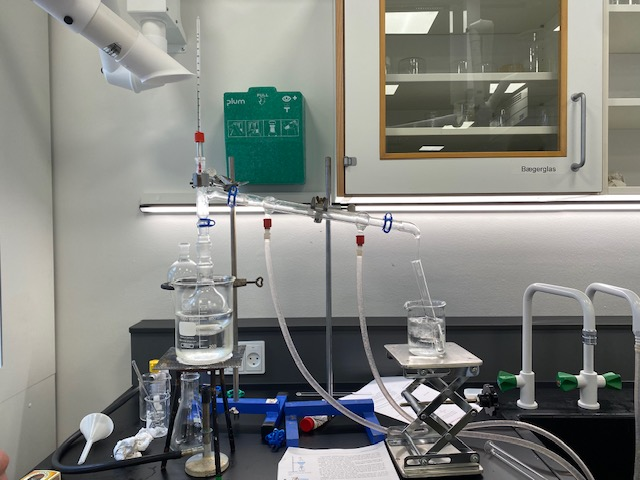
\includegraphics[width=\textwidth]{Destillation.jpeg}}

\begin{document}
\maketitle
\section*{Formål}%
  \label{sec:Formål}
Formålet med eksperimentet er fremstilling af 2-chlor-2-methylpropan ved sammenblanding af 2-methylpropan-2-ol med koncentreret saltsyre, hvorefter produktet isoleres gennem forskellige processer, herunder en destillation.

\section*{Teori}%
  \label{sec:Teori}
Ved blandingen af 2-methylpropan-2-ol og koncentreret saltsyre sker reaktionen i \cref{fig:subst}.
Denne er en substitutionsreaktion. 
Substitutionsreaktioner defineres ved, at der udskiftes et atom eller en atomgruppe med et andet atom eller atomgruppe. 
Siden en forudsætning for dette er, at bindinger brydes, kræver det som regel tilførsel af energi i form af eksempelvis lys eller varme.
\begin{figure}[H]
\begin{center}
  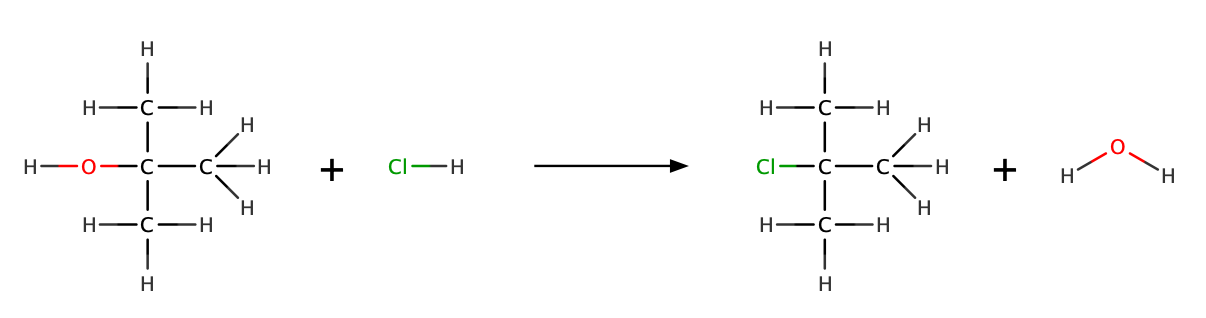
\includegraphics[scale=0.3]{Subst.png}
\end{center}
\caption{Substitutionsreaktion tegnet i MarvinSketch}
\label{fig:subst}
\end{figure}

Kogepunktet for 2-chlor-2-methylpropan er $50,8 \;\unit{\celsius} $, hvilket nemt kan bekræftes ved opslag i en databog.
Dette passer med, at hovedløbet opsamles i temperaturintervallet fra \qty{48}{\celsius} til \qty{53}{\celsius}.

Under Udførelse påstår vi, at reaktionsblandningen deler sig i to faser ved substitutionsreaktionen.
Dette vil vi nu redegøre for.
Vi har anvendt et overskud af \ce{HCl} (se Efterbehandling), så der vil også være \ce{HCl} i reaktionsblandningen.
Ved at kigge på eletronegativitetsforskellen på \ce{H} og \ce{Cl}, ved vi, at bindingen mellem dem er en polær elektronparbinding, siden $\Delta EN=0,9$.
Altså må molekylet være polært.
Ved at kigge på strukturformlen for 2-chlor-2-methylpropan, ser vi, at det ingen hydrofile grupper indeholder. 
Derimod indeholder det 3 \ce{C}-atomer med hydrofobe grupper.
Siden vi ved, at kun stoffer, som ligner hinanden, kan opløses i hinanden, kan vi konstatere, at reaktionsblandningen må dele sig i to faser.

Ved udrystningen med \ce{NaHCO3}-opløsningen (se Udførelse), sker reaktionen, hvis reaktionsskema er nedenfor i (1).
\begin{equation}
\begin{split}
  \ce{HCl + NaHCO3 -> H2O + CO2}
\end{split}
\end{equation}
Det er da sådan resterne af \ce{HCl} fjernes i forsøget.
Ved reaktionen dannes der \ce{H2O}, og væsken vil da dele sig i to faser igen, da 2-chlor-2-methylpropan jo ikke kunne opløses i vand. 
Det er den nederste fase, som er vand, grundet densiteterne for de to stoffer:
\begin{equation*}
\begin{split}
  \rho(\ce{H2O}) &= 1,00 \;\unit{g/mL} \\ 
  \rho(\ce{2-chlor-2-methylpropan}) &= 0,85 \;\unit{g/mL} 
\end{split}
\end{equation*}

\section*{Apparatur, kemikalier og sikkerhed}%
  \label{sec:Apparatur, kemikalier og sikkerhed}
\subsection*{Apparatur}%
  \label{sub:Apparatur}
 \begin{itemize}
  \item Måleglas, $25 \;\unit{mL} $ 
\item Måleglas, $50 \;\unit{mL} $ 
\item Måleglas, $100 \;\unit{mL} $ 
  \item Konisk kolbe, $250 \;\unit{mL} $ 
  \item Skilletragt, $250 \;\unit{mL} $ 
  \item Bægerglas, $100 \;\unit{mL} $ 
\item  Bægerglas, $250 \;\unit{mL} $ 
\item  Bægerglas, $400 \;\unit{mL} $ 
\item  Bægerglas, $1 \;\unit{L} $ 
\item Vat
\item Stativ 
\item Stativring til skilletragt 
\item 2 reagensglas 
\item Reagensglasstativ 
\item Spatel 
\item Vejebåd 
\item Pimpsten 
\item Tragt 
\item Filtrerpapir 
\item Bunsenbrænder 
\item Trefod med trådnet 
\item Vægt 
   \item Destillationsopstilling  
 \end{itemize} 
\subsection*{Kemikalier}
\begin{itemize}
  \item 2-methylpropan-2-ol
  \item Konc. saltsyre, \ce{HCl}
  \item 5 \% opløsning af natriumhydrogencarbonat, \ce{NaHCO3} 
\item Vandfrit natriumsulfat, \ce{Na2SO4} 
\item Isterninger
\end{itemize}
\subsection*{Sikkerhed}
\begin{itemize}
  \item 2-methylpropan-2-ol og 2-chlor-2-methylpropan er brandfarlige og farlige ved indånding.
  \item Konc. saltsyre kan forårsage alvorlige ætsninger og irritere luftvejene ved indånding.
\end{itemize}

\section*{Udførelse}
2-methylpropan-2-ol smeltes ved anbringelse i lunkent vand eller ved at lade flasken stå et lunt sted i en dags tid.
I et stinkskab blandes $20 \;\unit{mL} $ 2-methylpropan-2-ol og $60 \;\unit{mL} $ koncentreret saltsyre i en $250 \;\unit{mL} $ konisk kolbe.
Kolben lukkes med en vatprop, hvorefter den rystes forsigtigt under udsugning i ti minutter.

Væskebladningen hælden derefter over i en skilletragt i en stativring med et bægerglas under som i \cref{fig:skilletragt}.
Blandingen deler sig i to faser efter nogle minutter, hvor den nederste fase, som består af saltsyre, tappes og kasseres.
Rester af \ce{HCl} fjernes ved tilsætning af cirka $50 \;\unit{mL} $ 5\% \ce{NaHCO3}-opløsning til skilletragten, hvorefter denne rystes forsigtigt uden prop indtil størstedelen af \ce{CO2}-udviklingen er overstået. 

Proppen sættes herefter i, hvorefter skilletragten vendes skråt på hovedet.
Hanen lukkes op, så der lukkes luft ud.
Skilletragten rystes så forsigtigt, hvorefter hanen lukkes op igen.
Denne proces gentages indtil der næsten ingen luft lukkes ud længere.
Skilletragten hænges herefter op i ringen igen, hvor den nederste fase tappes og kasseres.
\begin{figure}[H]
\begin{center}
  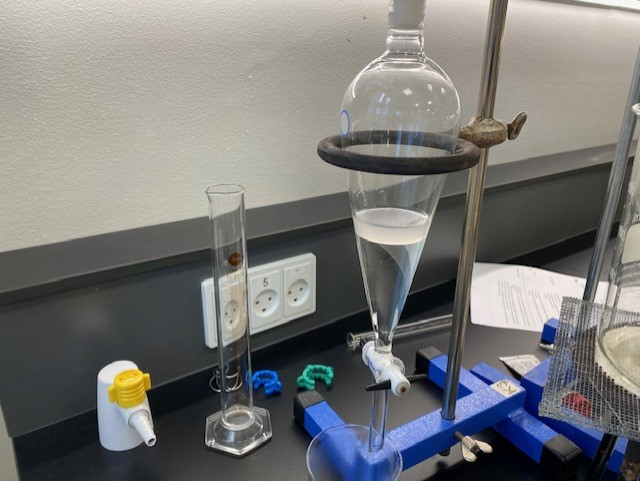
\includegraphics[scale=0.5]{Skilletragt}
\end{center}
\caption{Skilletragt ophængt i et stativ}
\label{fig:skilletragt}
\end{figure}

Den resterende fase tappes så ned i et $100 \;\unit{mL} $ bægerglas, hvor der tilet par gram vandfrit natriumsulfat for at fjerne vandrester.
Der røres så rundt med en spatel i et par minutter.

Væsken skal nu destilleres i opstillingen vist i \cref{fig:destillation}.
Opstilling stilles op med isvand i det lille bægerglas med et ekstra afvejet reagensglas klar til brug.
Væsken hældes ned i destillationskolben gennem en tragt med filtrerpapir.
Et par pimpsten tilsættes, hvorefter der åbnes for kølevandet til svaleren. 
Opvarmningen af vandbadet kan nu startes.

Et forløb opsamles indtil temperaturen er steget til cirka $\qty{48}{\celsius}$.
Herefter skiftes reagensglasset ud med det ekstra afvejede reagensglas, hvori hovedløbet opsamles i temperaturintervallet fra \qty{48}{\celsius} til \qty{53}{\celsius}.
Når destillationen er afsluttet, afbrydes opvarmningen og kølevandet. 
Ydersiden af reagensglasset med hovedløbet tørres af og reagensglasset vejes så.
\begin{figure}[H]
\begin{center}
  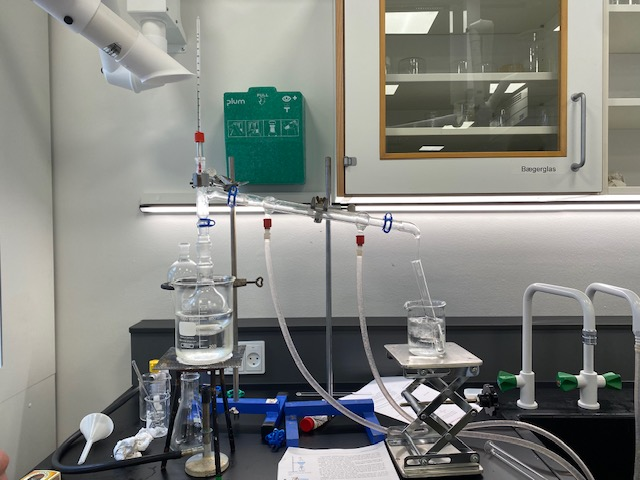
\includegraphics[scale=0.5]{Destillation.jpeg}
\end{center}
\caption{Destillationsopstillingen}
\label{fig:destillation}
\end{figure}

\section*{Resultater}
De afmålte værdier fremgår af nedenstående tabel.
\begin{table}[H]
\begin{tabular}{|l|l|}
\hline
$m(\text{reagensglas})$ & $m(\text{reagensglas og hovedløb})$ \\ \hline
25,742 g                & 34,176 g                            \\ \hline
\end{tabular}
\end{table}

\section*{Efterbehandling og sammenfatning af resultaterne}
Vi vil i efterbehandlingen beregne det praktiske udbytte i \% af det teoretiske udbytte.

Siden koncentreret saltsyre er en 37\% (masseprocent) opløsning af \ce{HCl} i vand med densiteten $1,19 \;\unit{g/mL} $, og vi har anvendt $60 \;\unit{mL} $ konc. saltsyre, så må massen af den anvendte \ce{HCl} være følgende.
\begin{equation*}
\begin{split}
  m(\ce{HCl})&=c_{masse\%}(\ce{HCl}) \cdot V(opløsning) \cdot \rho(opløsning) \\
  &=0,37 \cdot 60 \;\unit{mL} \cdot 1,19 \;\unit{g/mL  } \\
  &= 26,418 \;\unit{g}  
\end{split}
\end{equation*}
Stofmængden af den anvendte \ce{HCl} er da
\begin{equation*}
\begin{split}
  n(\ce{HCl}) &= \frac{m(\ce{HCl})}{M(\ce{HCl})} \\ 
  &= \frac{26,418 \;\unit{g}  }{36,46 \;\unit{g/mol} }\\ 
  &= 0,7245749 \;\unit{mol}. 
\end{split}
\end{equation*}
Vi har anvendt $20 \;\unit{mL} $ 2-methylpropan-2-ol, der har densiteten $0,7887 \;\unit{g/mL } $. 
Massen er da
\begin{equation*}
\begin{split}
  m(\text{2-methylpropan-2-ol}) &= V(\text{2-methylpropan-2-ol}) \cdot \rho(\text{2-methylpropan-2-ol}) \\
  &= 20 \;\unit{mL} \cdot 0,7887 \;\unit{g/mL} \\ 
  &= 15,774 \;\unit{g} 
\end{split}
\end{equation*}
Stofmængden kan da nu regnes.
\begin{equation*}
\begin{split}
  n(\text{2-methylpropan-2-ol}) &= \frac{m(\text{2-methylpropan-2-ol})}{M(\text{2-methylpropan-2-ol})} \\ 
  &= \frac{15,774 \;\unit{g}  }{74,12 \;\unit{g/mol} }\\ 
  &= 0,212412304\;\unit{mol} 
\end{split}
\end{equation*}
Fra substitutionsreaktionen i \cref{fig:subst}, kan det ses, at stofmængdeforholdet mellem 2-methylpropan-2-ol og \ce{HCl} er 1:1. 
Dog, siden $n(\ce{HCl})>n(\text{2-methylpropan-2-ol})$, er der anvendt et overskud af \ce{HCl}. 
I \cref{fig:subst} ses det også, at stofmængdeforholdet mellem 2-methylpropan-2-ol og 2-chlor-2-methylpropan er 1:1.
Derfor må følgende gælde.
\[
n(\text{2-chlor-2-methylpropan})=n(\text{2-methylpropan-2-ol})= 0,212412304\;\unit{mol} 
\] 
Derfor må det teoretiske udbytte af 2-chlor-2-methylpropan være
\begin{equation*}
\begin{split}
  m_{\text{teoretisk}}(\text{2-chlor-2-methylpropan})&= n(\text{2-chlor-2-methylpropan}) \cdot M(\text{2-chlor-2-methylpropan})\\ 
  &= 0,212412304\;\unit{mol} \cdot 92,57 \;\unit{g/mol} \\ 
  &=19,66300702 \;\unit{g} 
\end{split}
\end{equation*}
Det praktiske udbytte er da
\begin{equation*}
\begin{split}
  m_{\text{praktisk}}(\text{2-chlor-2-methylpropan})&=m(\text{reagensglas og hovedløb})-m(\text{reagensglas})\\
  &= 34,176 \;\unit{g} - 25,742 \;\unit{g} \\ 
  &= 8,434 \;\unit{g} 
\end{split}
\end{equation*}
Endeligt kan vi udregne det praktiske udbytte i \% af det teoretiske udbytte (2 betydende cifre).
\[
\frac{m_{\text{praktisk}}(\text{2-chlor-2-methylpropan})}{m_{\text{teoretisk}}(\text{2-chlor-2-methylpropan})}\approx 0,43 = 43\%
\] 
Altså er det praktiske udbytte 43 \% af det teoretiske udbytte.

\section*{Mulige fejlkilder}
Der er to iøjnefaldene mulige fejlkilder.
Den vigtigste er nok filtrerpapiret, hvorigennem chlorforbindelsen bliver hældt gennem.
En del af chlorforbindelsen kan mistes, da det ikke kommer med ned i destillationskolben.
Dette ville resultere i et mindre udbytte.
Det samme kan netop være tilfældet med hensyn til tapningen fra skilletragten, der også ville give et mindre udbytte.

\section*{Konklusion}
Vi har i eksperimentet fremstillet 2-chlor-2-methylpropan ved sammenblanding af 2-methylpropan-2-ol med koncentreret saltsyre ved processen beskrevet under 'Udførelse'.
Dette er gjort med et udbytte på 43 \%.

\end{document}
